\documentclass[aspectratio=43]{beamer}

\usetheme{CambridgeUS}
%\usepackage{amssymb,amsfonts,amsmath,cite,enumerate,float,indentfirst}
%\usepackage{amsmath}
\usepackage{sansmathaccent}
\usepackage[utf8]{inputenc}
\usepackage[english,russian]{babel}
\pdfmapfile{+sansmathaccent.map}
\usepackage{subfig}
\usepackage{appendixnumberbeamer}
\usepackage{booktabs}
\usepackage{xspace}
\usepackage{graphicx}
\usepackage{longtable}
\usepackage[scale=2]{ccicons}

\graphicspath{{Img/}}

\newcommand{\imgh}[5]{\begin{figure}[#5]\center{\includegraphics[width=#1]{#2}}\caption{#3}\label{fig:#4}\end{figure}}

\title[]{Численное моделирование корреляций между частицами от распада струнных кластеров при взаимодействии ядер высоких энергий}
%\subtitle{A modern beamer theme}
\date{4 июня 2019}
%\date{}
\author[]{Денис Ужва \\
	  Научный руководитель: д.ф.-м.н., профессор кафедры ФВЭиЭЧ Вечернин В.В.}
\institute[]{СПбГУ, кафедра физики высоких энергий и элементарных частиц}
% \titlegraphic{\hfill\includegraphics[height=1.5cm]{logo.pdf}}

\begin{document}

\maketitle

\begin{frame}{Table of contents}
  \setbeamertemplate{section in toc}[sections numbered]
  \tableofcontents[hideallsubsections]
\end{frame}



\section{Введение}

\begin{frame}{Струнная модель в КХД}
	
	Важным объектом в релтивистской квантовой хромодинамике является так называемая кварк-глюонная струна
	\begin{figure}[H]
		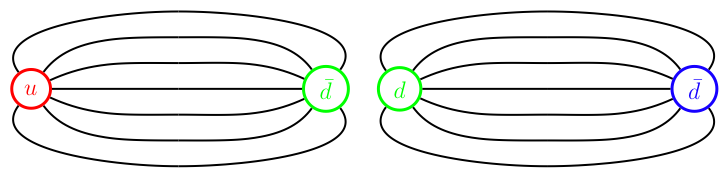
\includegraphics[width=\textwidth]{string}
		\caption*{Наивная модель поля сильного взаимодействии}
		\label{fig:fluctuations}
	\end{figure}

\end{frame}

\begin{frame}{Слияние струн}
	
	Рассеяние ядер при высоких энергиях подразумевает образование струн, которые перекрываются и сливаются до начала процесса адронизации
	\begin{figure}[H]
		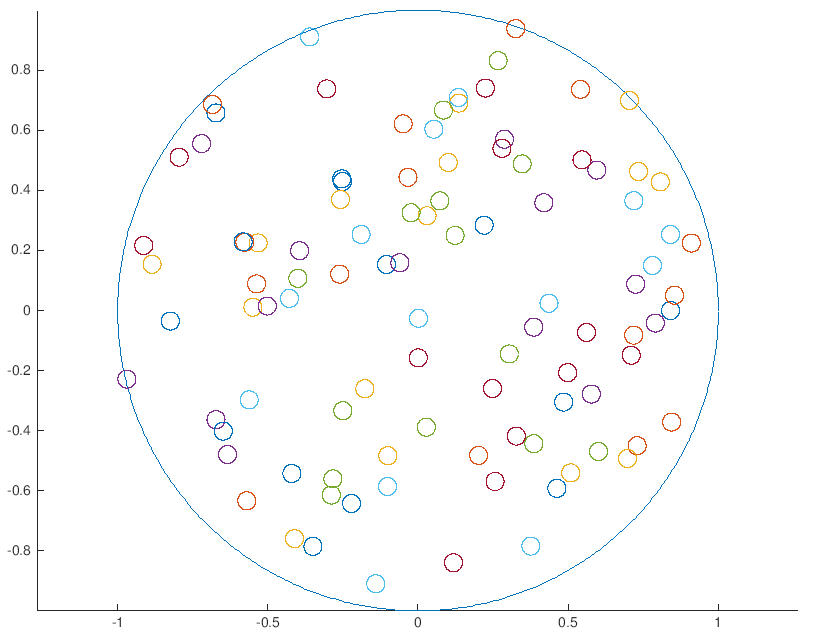
\includegraphics[width=0.5\textwidth]{interactionarea}
		\caption*{Визуализация струн в поперечном сечении ядер}
		\label{fig:interactionarea}
	\end{figure}

\end{frame}

\section{Модель непрерывного поперечного сечения}

\begin{frame}{Мотивация}
	
	\Large{
	\begin{itemize}[<+- | alert@+>]
		\item Непрерывная модель точнее, чем дискретная решётка
		\item До сего момента никто не проводил расчёт корреляций $p_t$ на непрерывном сечении
	\end{itemize}
	}

\end{frame}

\begin{frame}{Разработка генератора событий}

	Программа реализована на языке C++. Основные этапы расчёта:
	\begin{itemize}[<+- | alert@+>]
		\item Генерация центров струн в поперечном сечении
		\item Поиск кластеров, нахождение их площадей и подсчёт количества струн 
		\item Генерация значений множественности и поперечного импульса
		\item Расчёт корреляционного коэффициента
	\end{itemize}

\end{frame}

\begin{frame}{Генерация множественности и попереного импульса}

	Множественность рождённых частиц (из кластера $k$) генерировалась с помощью распределения Пуассона со следующим средним:
	\begin{align*}
		\langle n \rangle_k = \mu_0 \sqrt{\frac{N_k S_k}{\sigma_0}},
	\end{align*}
	а поперечный импульс -- по Гауссу, сразу для всего события $i$:
	\begin{align*}
		f((p_t)_i^F) = \frac{1}{\sqrt{2\pi} \sigma_{(p_t)_i^F}} \exp{\left( - \frac{((p_t)_i^F - \overline{(p_t)_i^F})^2}{2(\sigma_{(p_t)_i^F})^2} \right)}, \qquad \qquad \quad \\
		\overline{(p_t)_i^F} = \frac{\overline{p}}{n_i^F} \sum_{k = 1}^{M_i} n_k \sqrt[4]{\eta_k} = \overline{p} \cdot p_\Sigma, \quad 
		\sigma_{(p_t)_i^F}^2 = \frac{\sigma_p^2}{(n_i^F)^2} \sum_{k = 1}^{M_i} n_k \sqrt{\eta_k} = \sigma_p^2 \cdot \sigma_\Sigma^2.
	\end{align*}

\end{frame}

\begin{frame}{Расчёт корреляционного коэффициента}

	Коррелятор показывает зависимость величин в переднем и заднем быстротных окнах. Для множественности и попереного импульса он вычисляется по следующим формулам:
	\begin{align*}
		b_{nn} = \frac{\langle n_F n_B \rangle - \langle n_F \rangle \langle n_B \rangle}{\langle n_F^2 \rangle - \langle n_F \rangle^2}, \\
		b_{p_tp_t} = \frac{\langle p_F p_B \rangle - \langle p_F \rangle \langle p_B \rangle}{\langle p_F^2 \rangle - \langle p_F \rangle^2}.
	\end{align*}
	
\end{frame}

\begin{frame}{Предельный случай большой плотности струн}

	При большой плотности струн значения коэффициентов корреляции выходят на асимптотические кривые: 
	\begin{align*}
		b_{nn} = \frac{1}{1 + 4 \cdot \sqrt{\langle \eta \rangle}}, \quad \\
		b_{p_tp_t} = \frac{1}{1 + 16 \cdot \gamma^2 \cdot \sqrt{\langle \eta \rangle}}.
	\end{align*}
	
\end{frame}

\section{Результаты}

\begin{frame}{Влияние слияния струн на множественность}
	
	Как видно на следуюшем графике, учёт влияния слияния струн уменьшает прирост множественности при увеличении плотности струн:
	\begin{figure}[H]
		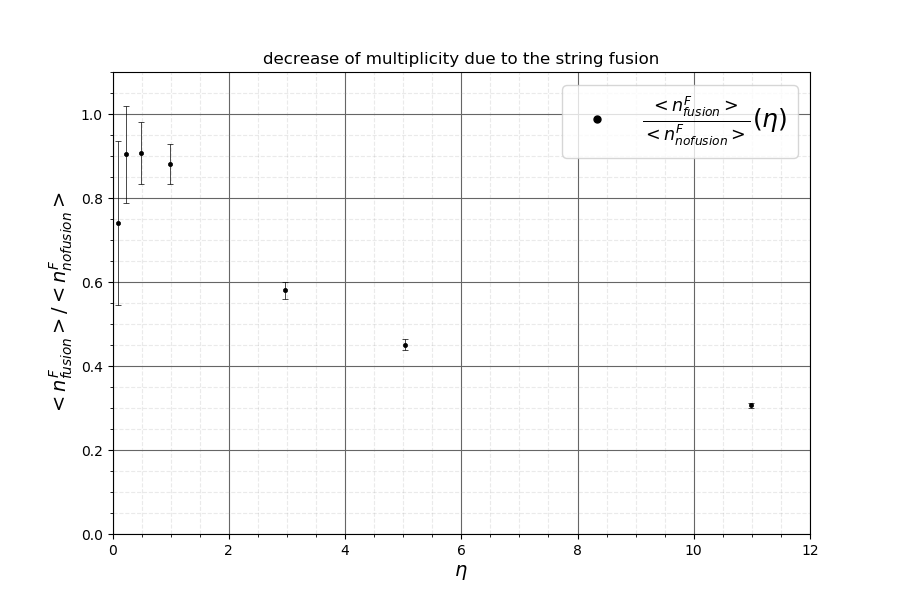
\includegraphics[width=0.7\textwidth]{nn0eta}
		\caption*{Зависимость $\langle n_{f} \rangle / \langle n_{nf} \rangle$ от $\eta$}
		\label{fig:nn0eta}
	\end{figure}

\end{frame}

\begin{frame}{Зависимость $b_{nn}$ от средней плотности струн $\langle \eta \rangle$}

	Коэффициент корреляции множественностей зависит от плотности струн как продемонстрировано на графике ниже
	\begin{figure}[H]
		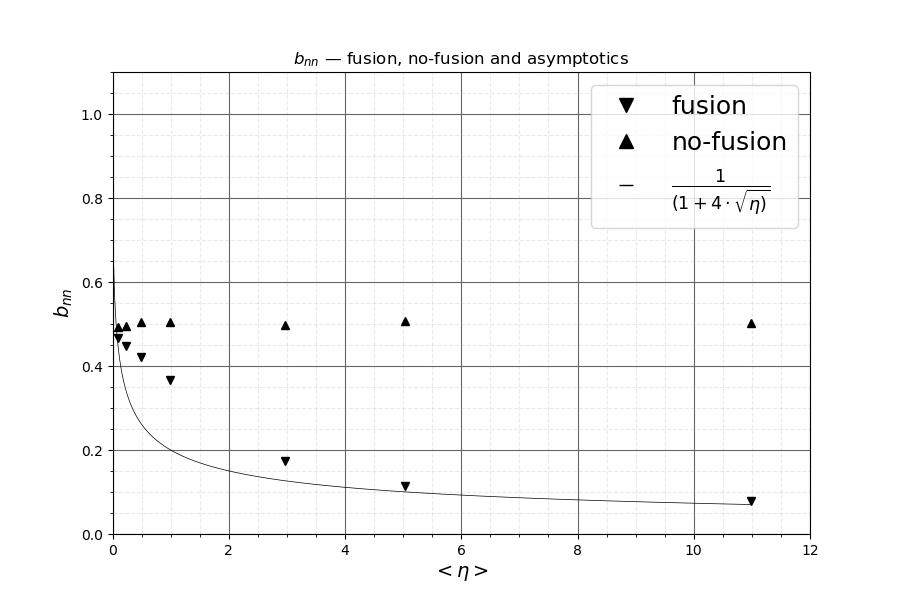
\includegraphics[width=0.7\textwidth]{b_nn}
		\caption*{Зависимость $b_{nn}$ от $\langle \eta \rangle$}
		\label{fig:b_nn}
	\end{figure}

\end{frame}

\begin{frame}{Зависимость $b_{p_tp_t}$ от средней плотности струн $\langle \eta \rangle$}

	Аналогичный график -- но уже для коэффициента корреляции поперечных импульсов
	\begin{figure}[H]
		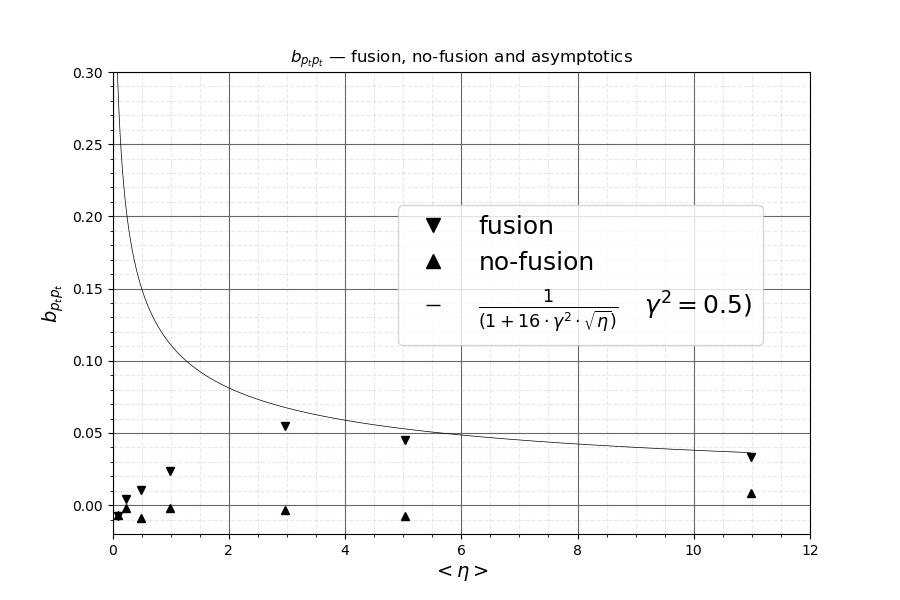
\includegraphics[width=0.7\textwidth]{b_pp}
		\caption*{Зависимость $b_{pp}$ от $\langle \eta \rangle$}
		\label{fig:b_pp}
	\end{figure}

\end{frame}

\section{Заключение}

\begin{frame}{Перспективы разработки генератора}

	\begin{itemize}[<+- | alert@+>]
		\item Применение распределения Вудса-Саксона для моделирования ядра
		\item Введение переменной центральности столкновения
		\item Оптимизация работы программы
		\item Применение к расчётам на реальных установках (NICA, LHC)
	\end{itemize}

\end{frame}

\end{document}

